\documentclass[10pt,a4paper]{article}
\usepackage[utf8]{inputenc}
\usepackage{amsthm}
\usepackage{amsmath}
\usepackage{float}
\usepackage{fancyhdr}
\usepackage{amsfonts}
\usepackage{amssymb}
\usepackage{algorithmic}
\usepackage{url}
\usepackage{hyperref}
\usepackage[pdftex]{graphicx}

\title{NetSec - Exercise 02} %\LaTeX
\author{\textbf{Che-Hao Kang, Aman Azim}} %\footnote{he is TA}
\date{\today} 
\begin{document} 
\maketitle 

\subsection*{Task 2.3 (practical): Website Login credentials}
From \textbf{\href{https://httpd.apache.org/docs/2.4/misc/password\_encryptions.html}{Apache website}} , \textbf{\$apr1\$} passwords are generated by \textbf{MD5} and salts are included to have diverse passwords which is between two dollar(\textbf{\$}) signs. For example, in \textbf{netsec:\$apr1\$/pE9u4cQ\$ZfQfXfZ8NWh2gfFpIx22T0}, the salt is \textbf{/pE9u4cQ}.

Having this information in hand, we can use programming to import the document, extract English words and employ Linux command to produce all corresponding MD5 passwords. 

Once the MD5 password is the same as \textbf{\$apr1\$/pE9u4cQ\$ZfQfXfZ8NWh2gfFpIx22T0}, we are done!
  \begin{figure}[h]
    \begin{center}
      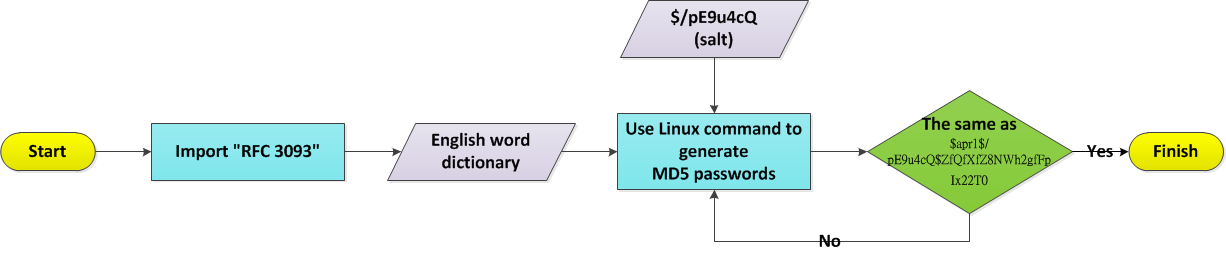
\includegraphics[width=1.0\textwidth]{practicalPic}
      \caption{Flow Chart of Our Approach}
      \vskip 0 pt
      \label{fig:practicalPic}
    \end{center}
  \end{figure}

\textsl{Programming details (\href{https://goo.gl/hvM4rt}{source code})} :

\begin{enumerate}
\item {first feature;}
\item {second feature;}
\item {everything is much easier to understand, and therefore, easier to implement correctly.}
\end{enumerate}

\begingroup
    \fontsize{10pt}{12pt}\selectfont
    \begin{verbatim}  
        % how to set font size here to 10 px ?  
    \end{verbatim}  
\endgroup
 
\end{document} 